\documentclass[11pt,a4paper]{article}

% --- packages -------------------------------------------------------------
\usepackage[utf8]{inputenc}
\usepackage[T1]{fontenc}
\usepackage{lmodern}
\usepackage{microtype}
\usepackage[a4paper,margin=2.4cm,headheight=14pt]{geometry}
\usepackage{amsmath,amssymb,mathtools}
\usepackage{graphicx}
\usepackage{booktabs}
\usepackage{tabularx}
\usepackage{array}
\usepackage{xcolor}
\usepackage{enumitem}
\usepackage{caption}
\usepackage{subcaption}
\usepackage[scaled=0.85]{beramono}
\usepackage{listings}
\usepackage{titling}
\usepackage{titlesec}
\usepackage{fancyhdr}
\usepackage[round,authoryear]{natbib}
\usepackage{hyperref}

% --- colors / theming -----------------------------------------------------
\definecolor{accent}{HTML}{0F5C8A}
\definecolor{accent2}{HTML}{C2410C}
\definecolor{rule}{HTML}{8895A1}
\definecolor{codebg}{HTML}{F5F7FA}
\definecolor{codekw}{HTML}{0F5C8A}
\definecolor{codestr}{HTML}{067D17}
\definecolor{codenum}{HTML}{C2410C}
\definecolor{codecom}{HTML}{6E7781}

\hypersetup{
  colorlinks=true,
  linkcolor=accent,
  urlcolor=accent,
  citecolor=accent,
  pdftitle={Wave-image generation in Python: a tooling survey},
  pdfauthor={HumanNatureAttunement},
}

\titleformat{\section}
  {\Large\bfseries\color{accent}}
  {\thesection}{0.6em}{}
  [{\color{rule}\titlerule[0.6pt]}]
\titleformat{\subsection}
  {\large\bfseries\color{accent}}
  {\thesubsection}{0.55em}{}

\lstdefinelanguage{pythonish}{
  morekeywords={def,class,return,if,else,elif,for,while,in,not,and,or,from,import,
                as,with,True,False,None,lambda,try,except,finally,pass,raise,
                yield,is,break,continue},
  morecomment=[l]\#,
  morestring=[b]",
  morestring=[b]'
}
\lstset{
  language=pythonish,
  basicstyle=\ttfamily\small,
  keywordstyle=\color{codekw}\bfseries,
  stringstyle=\color{codestr},
  commentstyle=\color{codecom}\itshape,
  numberstyle=\tiny\color{codecom},
  numbers=left, numbersep=8pt,
  backgroundcolor=\color{codebg},
  frame=single, framesep=4pt, framerule=0pt, rulecolor=\color{codebg},
  breaklines=true, breakatwhitespace=true,
  columns=fullflexible, keepspaces=true,
  xleftmargin=10pt, xrightmargin=4pt,
  aboveskip=8pt, belowskip=8pt,
}

\pagestyle{fancy}
\fancyhf{}
\fancyhead[L]{\small\color{rule}HNA -- Wave synthesis}
\fancyhead[R]{\small\color{rule}\thepage}
\renewcommand{\headrulewidth}{0pt}
\fancypagestyle{plain}{\fancyhf{}\fancyfoot[R]{\small\color{rule}\thepage}}

\setlength{\droptitle}{-1.4cm}

\title{\vspace{-1cm}\Huge\bfseries Wave-image generation in Python \\[2pt]
  \large\mdseries A tooling survey for parametric, reproducible
  ocean-stimulus synthesis}
\author{HumanNatureAttunement project \\[-2pt]
  \small Antoine Bellemare \& Mar Estarellas}
\date{\small \today}

\newcommand{\code}[1]{\texttt{\small #1}}

\begin{document}

\maketitle
\thispagestyle{plain}

\begin{abstract}\noindent
The HNA project couples brain / heart / muscle rhythms with the visual
envelope of natural sea waves. The complementary need is to \emph{generate}
sea-wave clips with precise, dialed-in oscillation properties so that
entrainment can be probed parametrically: ``does a 0.25\,Hz wave drive
respiration more than a 0.10\,Hz wave?'' This report surveys the
techniques available in 2026 to synthesise realistic, controllable
sea-wave images and video from Python; recommends a 3-tier pipeline that
spans the realism / cost trade-off; and gives the closed-form
wind-speed-to-wave-period relationship that lets us hit a chosen
neurophysiological target band ($0.1$--$0.5$\,Hz) directly.
\end{abstract}

\vspace{4pt}\hrule height 0.6pt
\vspace{6pt}{\small\color{rule}
This document compiles with \code{tectonic report/wave\_synthesis.tex}.
The figures are produced by \code{scripts/wave\_synthesis\_figures.py};
the small Tessendorf FFT ocean snapshots inside it are themselves a
working demo of the recommended Tier 1 pipeline.}
\vspace{6pt}\hrule height 0.6pt

\tableofcontents
\vspace{6pt}

% =========================================================================
\section{Why a synthesis module}
% =========================================================================

The analysis-side module \code{HNA.modules.video} reduces a sea-wave
\emph{recording} to a battery of 1-D signals (luminance envelope,
optical-flow magnitude, modal coefficients, per-pixel temporal spectra,
windowed complexity). This survey is the symmetric question: how do we
\emph{produce} sea-wave clips for which the wave period, foam content,
fetch, depth, viewing angle and lighting are all known and controllable
ahead of recording?

\paragraph{Why this matters.} Naturalistic stimuli capture richer
neurophysiological responses than artificial gratings, but they sacrifice
parametric control. Synthesis closes the gap: a procedurally generated
ocean clip is naturalistic \emph{and} fully parameterised. With an
explicit dominant frequency $f_p$ we can:
\begin{itemize}[leftmargin=1.5em,itemsep=0.4em]
  \item map dose-response curves of EEG envelope coupling vs.\ $f_p$
        within the autonomic / respiration band;
  \item match audio and visual envelopes by construction (test
        cross-modal entrainment without confounds);
  \item run condition replicates from a fixed seed for reproducibility.
\end{itemize}

\paragraph{Constraints.} Whatever pipeline we adopt must (i)~accept
explicit numerical inputs (wind, fetch, depth, choppiness, foam, sun, camera, seed)
rather than text prompts, (ii)~run on Windows + CUDA with permissive
licensing, and (iii)~deliver MP4 at 30\,fps for $\sim$60--120\,s. These
constraints rule out most generative-AI pipelines (Sec.~\ref{sec:ai}) and
favour spectrum-based procedural synthesis with optional photoreal
rendering.

% =========================================================================
\section{Families of techniques}
% =========================================================================

% -------------------------------------------------------------------------
\subsection{Procedural mathematical surfaces}
% -------------------------------------------------------------------------

The dominant family in computer graphics for open-water animation since
the 1980s. A heightfield $\eta(x, y, t)$ is computed analytically and
rendered with shader code; no fluid PDE is solved.

\paragraph{Sum of sines and Gerstner waves.} The simplest sum,
\begin{equation}
  \eta(x, y, t) = \sum_{i=1}^{M} a_i \sin(\mathbf{k}_i \cdot \mathbf{x} - \omega_i t + \phi_i),
\end{equation}
is fast and trivially controllable but flat-crested and unconvincing.
\citet{fournier1986} introduce trochoidal (Gerstner) waves, which add a
horizontal displacement so crests sharpen:
$\mathbf{x} \to \mathbf{x} - (\mathbf{k}_i / k_i) Q_i a_i \sin(\dots)$.
\citet{finch2004} (\emph{GPU Gems} ch.~1) gives the standard recipe.
Dispersion $\omega = \sqrt{g k \tanh(k h)}$ couples wavenumber to depth.

\paragraph{Spectrum-based / Tessendorf FFT ocean.} The state of the art
for offline open-water (Pixar, Weta, EA, Unreal) since
\citet{tessendorf2001}. A 2-D wavenumber grid is sampled from a
sea-surface spectrum -- typically Phillips, Pierson--Moskowitz
\citep{pierson1964}, or JONSWAP \citep{hasselmann1973} -- multiplied by
time-evolved phasors $\exp(i \omega(\mathbf{k}) t)$, and inverse-FFTed to
a tileable heightfield (Fig.~\ref{fig:spectra}). Choppy waves are added
by horizontally displacing the gradient field; foam is detected as the
zero-set of the displacement Jacobian. The pipeline is
\citep{mastin1987}-style and amounts to $\sim$200 lines of NumPy/CuPy
(see Fig.~\ref{fig:fft-ocean}, where the snapshots are produced by
\code{scripts/wave\_synthesis\_figures.py}).

\begin{figure}[ht]
  \centering
  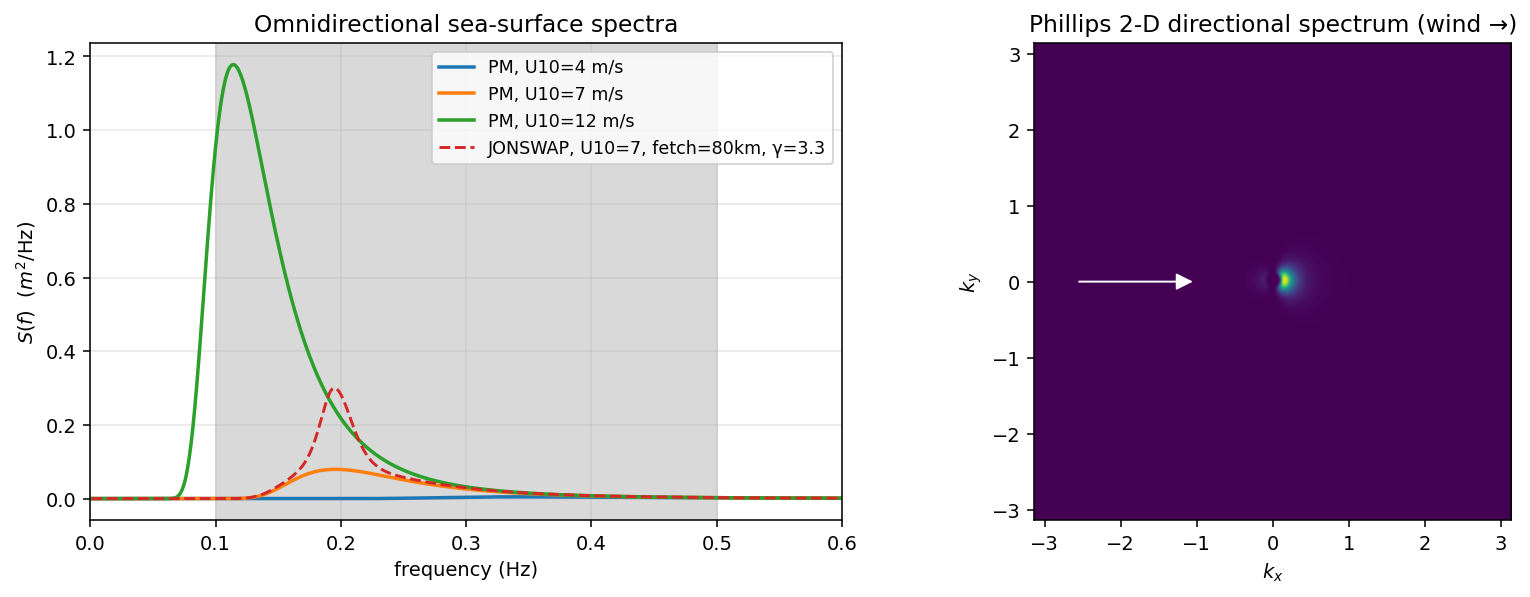
\includegraphics[width=\linewidth]{figures/pm_spectrum.png}
  \caption{Left: omnidirectional Pierson--Moskowitz frequency spectra at
  three wind speeds, plus a JONSWAP variant for fetch-limited seas. The
  shaded band is the target neurophysiological range
  ($0.1$--$0.5$\,Hz). Right: the corresponding 2-D directional Phillips
  spectrum used inside \citet{tessendorf2001}'s FFT ocean.}
  \label{fig:spectra}
\end{figure}

\begin{figure}[ht]
  \centering
  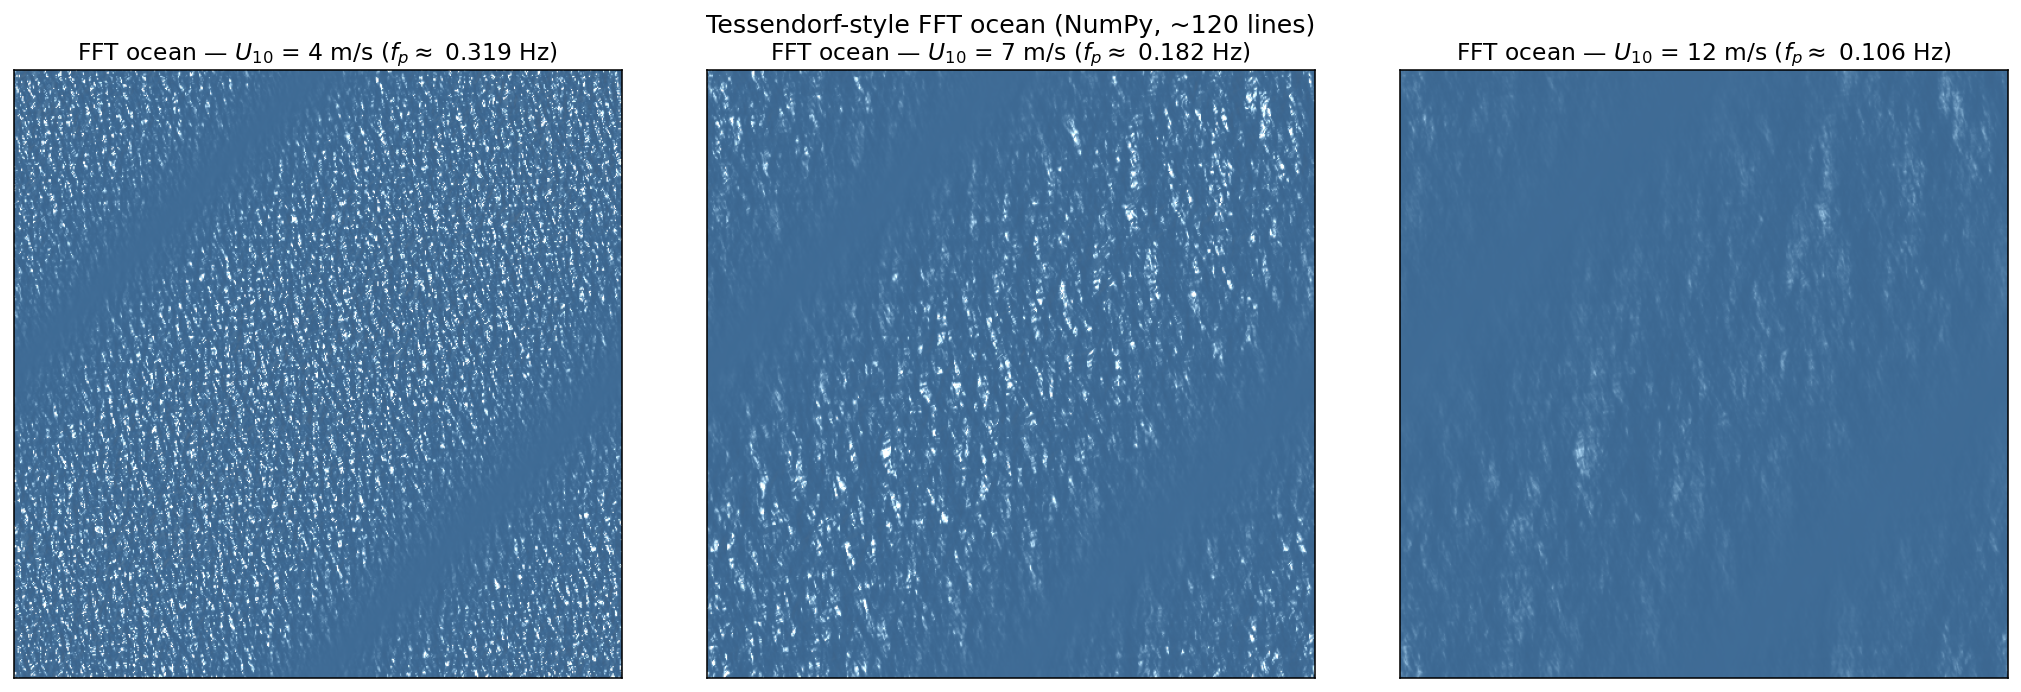
\includegraphics[width=\linewidth]{figures/fft_ocean_snapshots.png}
  \caption{Tessendorf-style FFT ocean rendered with $\sim$120 lines of
  NumPy + cheap Lambertian shading. Three wind speeds, same seed; peak
  period varies from $\sim$3\,s ($U_{10}$=4\,m/s) to $\sim$9\,s
  ($U_{10}$=12\,m/s). With proper sky / specular shading and a foam
  layer this approach is the workhorse of the visual-effects industry.}
  \label{fig:fft-ocean}
\end{figure}

\paragraph{Knobs the user controls.} For Tessendorf-FFT:
$U_{10}$ (wind speed at 10\,m), wind direction, fetch (JONSWAP),
gravity $g$, depth $h$, patch size $L$, grid resolution $N$,
choppiness $\lambda$, foam threshold, RNG seed.

\paragraph{Python implementations.}
\begin{itemize}[leftmargin=1.5em,itemsep=0.3em]
  \item \textbf{NumPy / CuPy from scratch.} $\sim$200 lines. Deterministic;
        easy to validate spectrally; runs in seconds on a CUDA GPU.
  \item \textbf{Taichi-lang} \citep{hu2019} ships an FFT ocean example;
        Python-first, JIT-compiled to CUDA; reproducible via
        \code{ti.init(random\_seed=...)}.
  \item \textbf{Mitsuba 3} \citep{mitsuba3} can render the heightfield
        (or its displacement map) with path-traced water; pure Python,
        BSD-3, CUDA via \code{LLVM}/\code{OptiX}.
\end{itemize}

% -------------------------------------------------------------------------
\subsection{Physics-based fluid simulation}
% -------------------------------------------------------------------------

Solve Navier--Stokes (or shallow-water, or SPH) on a grid and render the
result. \emph{For open-water visuals this is overkill} -- the
spectrum-based methods produce indistinguishable images at a tiny
fraction of the cost. Worth knowing about if shore-break / splash
close-ups matter later.

\begin{itemize}[leftmargin=1.5em,itemsep=0.3em]
  \item \textbf{Eulerian Navier-Stokes:} \emph{Stable Fluids} \citep{stam1999};
        \code{PhiFlow} \citep{phiflow} (Apache, JAX/PyTorch);
        \code{jax-cfd} (Apache).
  \item \textbf{SPH:} \code{PySPH} (BSD, slow);
        \code{Genesis} \citep{genesis} (Apache, GPU, 2024+).
  \item \textbf{Position-based fluids:} \citet{macklin2013}; bindings via
        \code{NVIDIA Flex} or \code{Taichi MPM}.
  \item \textbf{Lattice Boltzmann:} \code{lettucecfd/lettuce} (PyTorch, MIT).
\end{itemize}

\paragraph{Cost.} Anywhere from seconds (2-D shallow-water) to minutes
per frame (3-D NS with free surface). Realism depends almost entirely on
the rendering layer, not the solver.

% -------------------------------------------------------------------------
\subsection{GPU shader synthesis from Python}
% -------------------------------------------------------------------------

Write a fragment shader (typically a raymarched water surface) and run it
off-screen, dumping frames to MP4. Real-time even at 1080p.

\begin{itemize}[leftmargin=1.5em,itemsep=0.3em]
  \item \textbf{moderngl} (MIT) -- the canonical OpenGL bindings; load a
        GLSL shader, render to an offscreen FBO, capture frames via
        \code{imageio-ffmpeg}.
  \item \textbf{wgpu-py} (BSD) -- modern WebGPU bindings; future-proof.
  \item \textbf{Taichi} -- Python-first, JIT-to-CUDA, also runs on Apple
        Metal; particularly clean for a Tessendorf FFT ocean.
\end{itemize}

\paragraph{What to port.} Inigo Quilez's \emph{Seascape} Shadertoy (MIT)
is the standard reference shader; it raymarches a heightfield built from
nested noise + Gerstner waves, then shades with sky and Schlick Fresnel.
\citet{horvath2015} extends with empirical directional spectra. All
parameters are uniforms and trivially settable from Python.

% -------------------------------------------------------------------------
\subsection{AI / generative video synthesis}\label{sec:ai}
% -------------------------------------------------------------------------

The newest family and the most tempting for naturalistic stimuli, but the
worst fit for our use case for one structural reason: \emph{text- and
image-conditioned diffusion models do not let you specify a dominant
oscillation frequency}.

\begin{itemize}[leftmargin=1.5em,itemsep=0.3em]
  \item \textbf{Image:} Stable Diffusion + ControlNet via
        \code{diffusers} (Apache); produces stunning seascapes from a
        prompt but each frame is independent.
  \item \textbf{Video diffusion:} Stable Video Diffusion
        (Stability, \emph{non-commercial} license -- caveat for research
        outputs); AnimateDiff (Apache); CogVideoX
        \citep{cogvideox} (Apache, 2024); Open-Sora (Apache, 2024);
        HunyuanVideo, Lumina-Video.
  \item \textbf{Cinemagraphs.} \citet{holynski2021} animate water in a
        \emph{single} still photo by warping along a learned (or
        user-painted) Eulerian motion field; the result loops smoothly
        but the temporal frequency emerges from the model and the
        painted field rather than from a numerical knob.
  \item \textbf{Diffusion-based fluids.} A small but growing literature
        (e.g.\ DiffusionPDE) -- not a production tool yet.
\end{itemize}

\paragraph{Verdict for entrainment work.} Use these only as a stylistic
finish on top of a procedurally generated clip whose dominant frequency
has already been validated spectrally; never as the source of $f_p$.

% -------------------------------------------------------------------------
\subsection{Hybrid \& specialised}
% -------------------------------------------------------------------------

\begin{itemize}[leftmargin=1.5em,itemsep=0.3em]
  \item \textbf{Procedural geometry $\to$ photoreal renderer.}
        Generate FFT/Gerstner heightfield in Python, feed it to
        \citep{mitsuba3} (BSD-3, Python-first) or \textbf{Blender Cycles}
        via \code{bpy} (GPL) for path-traced output. The
        \emph{highest-realism reproducible} path.
  \item \textbf{Eulerian video magnification, in reverse.}
        \citep{wu2012,wadhwa2013} amplify tiny oscillations; the same
        decomposition can \emph{inject} a chosen frequency into an
        existing seascape video by modulating a phase-decomposed steerable
        pyramid. Niche but useful when you want to imprint, e.g., 0.2\,Hz
        on real footage.
  \item \textbf{Houdini Python.} Industry standard FX, but commercial
        license; HQueue scripting works but heavyweight.
  \item \textbf{Blender ``Ocean'' modifier.} Implements
        \citet{mastin1987} + Tessendorf choppiness + foam. Fully
        scriptable from \code{bpy}: knobs are \code{spatial\_size},
        \code{resolution}, \code{wind\_velocity}, \code{depth},
        \code{choppiness}, \code{foam\_coverage}, \code{random\_seed},
        animated over \code{time}. Renders with Cycles
        (path-traced, CUDA/OptiX) or Eevee (real-time-ish). \emph{The
        single best off-the-shelf option for this project.}
\end{itemize}

% -------------------------------------------------------------------------
\subsection{Rendering hosts callable from Python}
% -------------------------------------------------------------------------

\begin{tabularx}{\linewidth}{l l X}
\toprule
\textbf{Host} & \textbf{Python} & \textbf{Notes} \\
\midrule
Blender Cycles / Eevee & \code{bpy} (PyPI, GPL) & Ocean modifier built-in,
  HDRI sky, foam shaders, headless via
  \code{blender --background --python}.\\
Mitsuba 3              & \code{mitsuba} (PyPI, BSD-3) & physically-based,
  differentiable, CUDA via \code{LLVM}; bring your own geometry.\\
PyVista                & \code{pyvista} (MIT)    & quick procedural
  meshes, not photoreal.\\
Three.js               & \code{pythreejs}        & awkward but possible
  with Playwright screenshots.\\
\bottomrule
\end{tabularx}

% =========================================================================
\section{Frequency-targeting cheat sheet}\label{sec:cheatsheet}
% =========================================================================

For a fully developed sea, the Pierson--Moskowitz peak frequency is
\citep{pierson1964}
\begin{equation}
  f_p \;\approx\; \frac{0.13\, g}{U_{10}}
  \quad\Longleftrightarrow\quad
  U_{10} \;\approx\; \frac{0.13\, g}{f_p}.
\end{equation}
This single relation lets us go from a desired neurophysiological target
band straight to an actionable wind-speed input
(Fig.~\ref{fig:fp-vs-U10}).

\begin{figure}[ht]
  \centering
  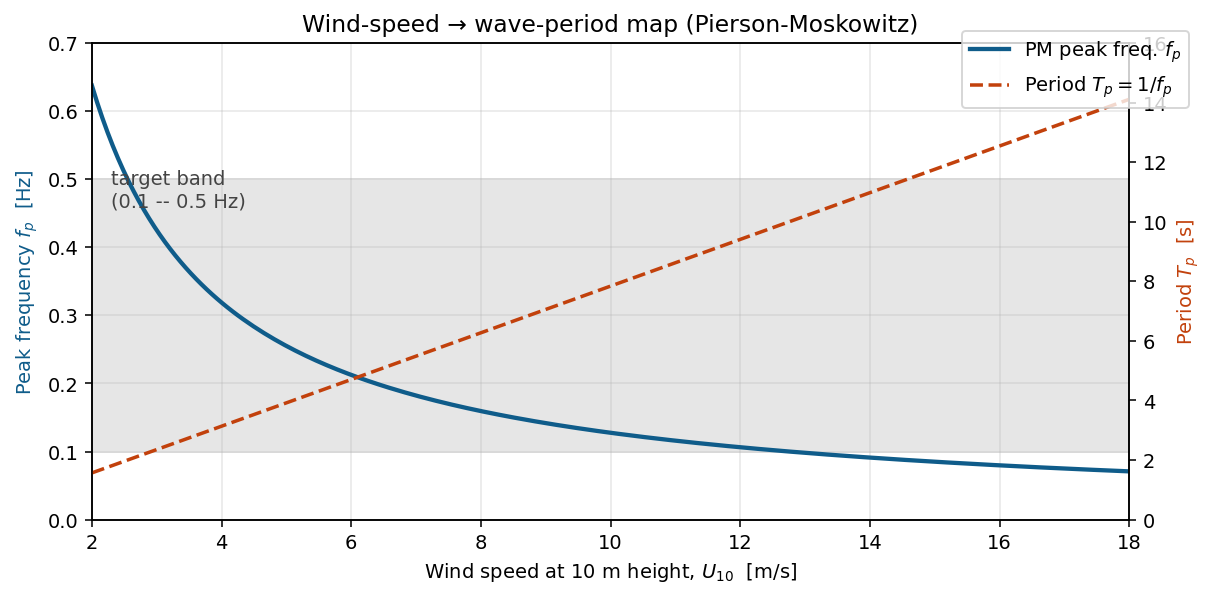
\includegraphics[width=0.95\linewidth]{figures/fp_vs_U10.png}
  \caption{Pierson--Moskowitz peak frequency $f_p$ and corresponding
  period $T_p = 1/f_p$ as a function of wind speed $U_{10}$. The shaded
  region marks the neurophysiological target band
  ($0.1$--$0.5$\,Hz). For $f_p = 0.25$\,Hz: $U_{10} \approx 5.1$\,m/s.
  For $f_p = 0.10$\,Hz (stormy swell): $U_{10} \approx 12.7$\,m/s.}
  \label{fig:fp-vs-U10}
\end{figure}

\begin{table}[ht]
\centering
\renewcommand{\arraystretch}{1.18}
\setlength{\tabcolsep}{8pt}
\begin{tabular}{@{}lll@{}}
\toprule
target $f_p$ (Hz) & target period $T_p$ (s) & $U_{10}$ (m/s, PM) \\
\midrule
0.10 (slow swell)   & 10.0 & 12.7 \\
0.15                & 6.7  &  8.5 \\
0.20                & 5.0  &  6.4 \\
0.25 (mid)          & 4.0  &  5.1 \\
0.33                & 3.0  &  3.8 \\
0.50 (small chop)   & 2.0  &  2.5 \\
\bottomrule
\end{tabular}
\caption{Wind-speed inputs that hit each entrainment-target frequency
under a fully developed Pierson--Moskowitz sea.}
\label{tab:cheat}
\end{table}

% =========================================================================
\section{Recommended pipeline tiers}
% =========================================================================

\begin{figure}[ht]
  \centering
  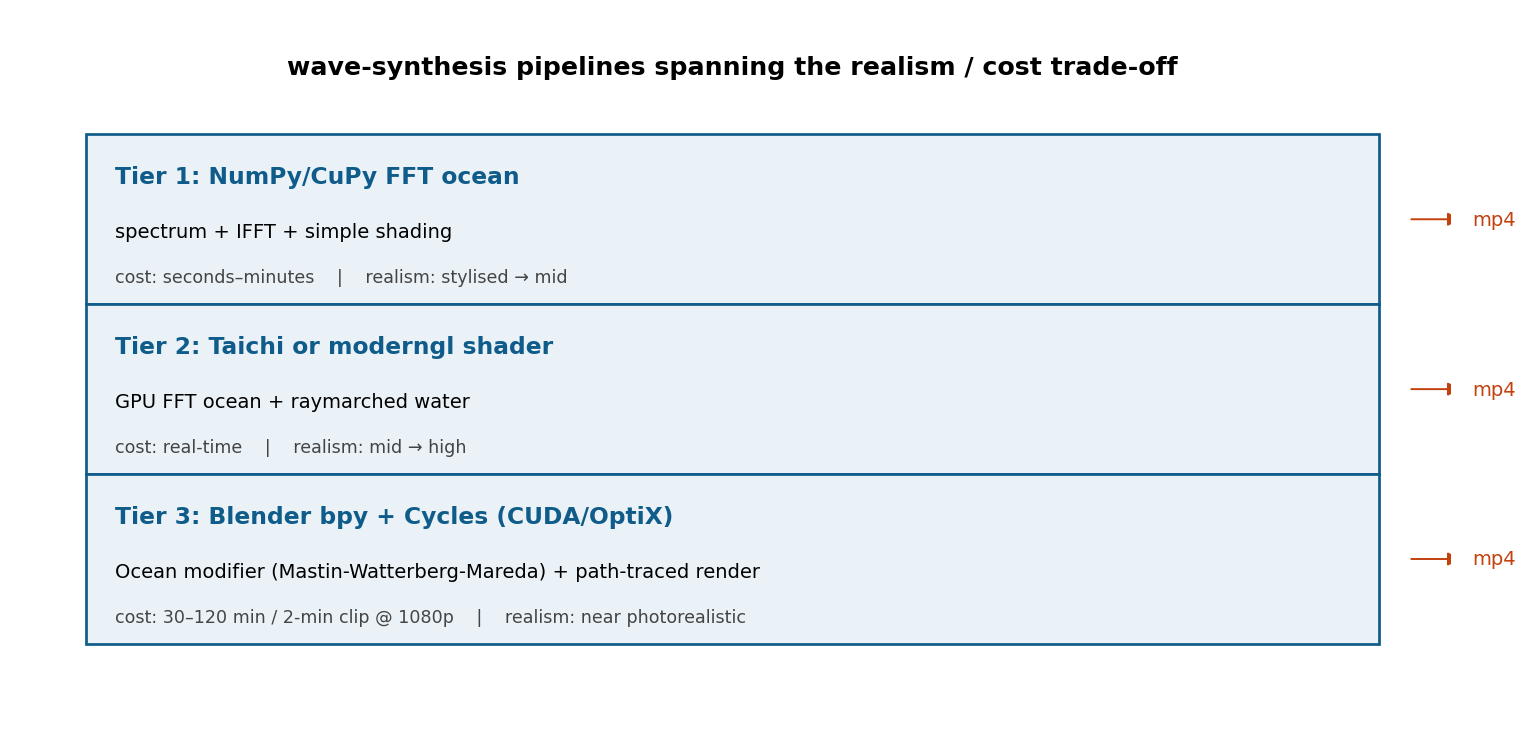
\includegraphics[width=\linewidth]{figures/pipeline_tiers.png}
  \caption{Three-tier wave-synthesis pipeline spanning the realism / cost
  trade-off. The same numerical knobs flow through all three; only the
  rendering layer changes.}
  \label{fig:tiers}
\end{figure}

\subsection{Tier~1 -- NumPy/CuPy FFT ocean (fastest)}

A $\sim$200-line implementation of \citet{tessendorf2001}: Phillips or
JONSWAP spectrum, time-evolved phasors, \code{numpy.fft.ifft2}, choppy
displacement, simple Blinn-Phong + sky shading, \code{imageio-ffmpeg}
for MP4. Already implemented as a demo in
\code{scripts/wave\_synthesis\_figures.py}. \textbf{Knobs:} $U_{10}$,
wind direction, fetch, depth $h$, choppiness, foam threshold, sun, camera,
seed. \textbf{Cost:} seconds to a few minutes for 30\,fps$\times$120\,s
$\times$1080p on a CUDA GPU. \textbf{Realism:} stylised but spectrally
correct.

\textbf{Use for:} pilot studies, parameter sweeps, dose-response curves
on $f_p$. The user changes a single argument ($U_{10}$) to walk through
Table~\ref{tab:cheat}.

\subsection{Tier~2 -- Taichi or moderngl shader (interactive)}

Same spectral inputs as Tier~1, but rendered in real-time with a Taichi
\citep{hu2019} kernel or a moderngl raymarched shader (Inigo Quilez's
\emph{Seascape} ported as a fragment shader). Render off-screen to a
PNG sequence, \code{ffmpeg} to MP4. \textbf{Use for:} interactive
parameter tuning before locking the final stimulus values.

\subsection{Tier~3 -- Blender bpy + Cycles (near photoreal)}

Drive Blender's \emph{Ocean} modifier from a Python script:

\begin{lstlisting}
import bpy

bpy.ops.mesh.primitive_plane_add(size=200)
plane = bpy.context.object
mod = plane.modifiers.new(name="Ocean", type='OCEAN')
mod.spatial_size   = 256
mod.resolution     = 32
mod.wind_velocity  = 5.1            # -> f_p ~ 0.25 Hz
mod.depth          = 200
mod.choppiness     = 1.0
mod.foam_coverage  = 0.4
mod.random_seed    = 42
mod.use_foam       = True

# Animate
scene = bpy.context.scene
scene.frame_start, scene.frame_end = 1, int(120 * 30)
scene.render.fps   = 30
scene.render.engine = 'CYCLES'
scene.cycles.device = 'GPU'

# Time keyframe
mod.time = 0
mod.keyframe_insert(data_path="time", frame=1)
mod.time = 120.0
mod.keyframe_insert(data_path="time", frame=scene.frame_end)

bpy.ops.render.render(animation=True)
\end{lstlisting}

Sky HDRI, sun position, camera, foam shader, and depth of field are all
scriptable. \textbf{Cost:} 30--120\,min for a 2-min 1080p clip on an
RTX-class GPU at moderate samples. \textbf{Realism:} near
photorealistic. \textbf{Use for:} the final experimental stimuli where
naturalistic appearance is itself a study variable.

\subsection{(Optional) Tier~4 -- Mitsuba 3 path-traced}

NumPy/Taichi FFT geometry exported as a displacement map, rendered with
\code{mitsuba 3}'s ocean BSDF + sky model. Use only if Cycles isn't
realistic enough for a particular shot. BSD-3, fully Python.

% =========================================================================
\section{Validation step (mandatory)}
% =========================================================================

Whichever tier we use, after rendering each clip we must verify that the
delivered dominant frequency matches the requested one. The
\code{HNA.modules.video} pipeline is exactly the right tool: run

\begin{lstlisting}
from HNA.modules.video import quantify_video
feats = quantify_video("synth/clip.mp4",
                       include_pixel_spectrum=True)
assert abs(feats.timestack.dominant_freq_hz - f_p_target) < 0.02
\end{lstlisting}

and confirm both the timestack peak and the modal $f_1$ land within
tolerance of the target $f_p$. The per-pixel spectrum's
\code{coherence\_index} should be high ($>0.9$ for a clean spectral
ocean). This validation step is doubly important if any AI rendering
pass is ever folded on top: that pass can shift phase, alias periods, or
introduce side-bands.

% =========================================================================
\section{What we will skip}
% =========================================================================

\begin{itemize}[leftmargin=1.5em,itemsep=0.4em]
  \item \textbf{Pure video-diffusion stimuli.} No reliable $f_p$ control;
        no reproducibility from a numerical seed alone. Useful only as a
        cosmetic finishing pass.
  \item \textbf{Full 3-D Navier--Stokes / SPH / MPM.} Gives nothing the
        spectral method doesn't already give for open-water; cost is
        $1000\times$ higher.
  \item \textbf{Houdini, Embergen.} Commercial; not portable.
\end{itemize}

% =========================================================================
\section{Proposed module skeleton (next step)}
% =========================================================================

The next deliverable is a module \code{HNA.modules.wave\_synth} structured
as:

\begin{lstlisting}
HNA.modules.wave_synth
+- spectra.py          # Phillips, PM, JONSWAP, dispersion
+- fft_ocean.py        # Tessendorf heightfield, choppy + foam
+- render_simple.py    # NumPy Blinn-Phong / sky shading -> mp4
+- render_taichi.py    # Taichi GPU shader (Tier 2)
+- render_blender.py   # bpy script template (Tier 3)
+- validate.py         # round-trip via HNA.modules.video
+- presets.py          # named (calm, swell, storm) parameter packs
\end{lstlisting}

with a single high-level entry point:

\begin{lstlisting}
from HNA.modules.wave_synth import synthesise

synthesise(out_mp4="stimuli/swell_025Hz.mp4",
           f_p_hz=0.25,                     # -> resolves U10 = 5.1 m/s
           duration_s=120, fps=30, resolution=(1920, 1080),
           tier="numpy",                    # or "taichi", "blender"
           wind_dir_deg=20, fetch_km=80, depth_m=200,
           choppiness=1.0, foam_coverage=0.4, sun_alt_deg=30,
           seed=42)
\end{lstlisting}

The \code{tier} argument selects the rendering backend; the spectral
parameters are identical across tiers, ensuring that the same $f_p$ can
be hit at three realism levels with one call.

% =========================================================================
\section*{References}
\addcontentsline{toc}{section}{References}
% =========================================================================

\begingroup
\renewcommand{\section}[2]{}
\begin{thebibliography}{99}\small

\bibitem[CogVideo Team(2024)]{cogvideox}
THUDM CogVideo team.
\newblock CogVideoX: Text-to-Video diffusion with an Expert Transformer.
\newblock GitHub: \url{https://github.com/THUDM/CogVideo}, 2024.

\bibitem[Finch(2004)]{finch2004}
M.~Finch.
\newblock Effective water simulation from physical models.
\newblock In \emph{GPU Gems}, ch.~1. Addison-Wesley, 2004.

\bibitem[Fournier \& Reeves(1986)]{fournier1986}
A.~Fournier, W.~T.~Reeves.
\newblock A simple model of ocean waves.
\newblock In \emph{SIGGRAPH '86}, pp.~75--84, 1986.

\bibitem[Genesis Team(2024)]{genesis}
Genesis-Embodied-AI.
\newblock Genesis: a generative \& universal physics engine.
\newblock GitHub: \url{https://github.com/Genesis-Embodied-AI/Genesis},
  2024.

\bibitem[Hasselmann \emph{et al.}(1973)]{hasselmann1973}
K.~Hasselmann \emph{et al.}
\newblock Measurements of wind-wave growth and swell decay during the
Joint North Sea Wave Project (JONSWAP).
\newblock \emph{Deutsche Hydrographische Zeitschrift}, A8(12), 1973.

\bibitem[Holm \emph{et al.}(2024)]{phiflow}
P.~Holzschuh \emph{et al.}
\newblock PhiFlow: a differentiable PDE simulation framework.
\newblock GitHub: \url{https://github.com/tum-pbs/PhiFlow}.

\bibitem[Holynski \emph{et al.}(2021)]{holynski2021}
A.~Holynski, B.~Curless, S.~Seitz, R.~Szeliski.
\newblock Animating pictures with Eulerian motion fields.
\newblock In \emph{CVPR}, 2021.

\bibitem[Horvath(2015)]{horvath2015}
C.~J.~Horvath.
\newblock Empirical directional wave spectra for computer graphics.
\newblock In \emph{Symposium on Digital Production}, 2015.

\bibitem[Hu \emph{et al.}(2019)]{hu2019}
Y.~Hu \emph{et al.}
\newblock Taichi: a language for high-performance computation on
spatially sparse data structures.
\newblock \emph{ACM TOG (SIGGRAPH Asia)}, 38(6):201, 2019.

\bibitem[Jakob \emph{et al.}(2022)]{mitsuba3}
W.~Jakob \emph{et al.}
\newblock Mitsuba 3 renderer.
\newblock \url{https://www.mitsuba-renderer.org/}.

\bibitem[Macklin \& M\"uller(2013)]{macklin2013}
M.~Macklin, M.~M\"uller.
\newblock Position based fluids.
\newblock \emph{ACM Trans.\ Graph.}, 32(4):104, 2013.

\bibitem[Mastin \emph{et al.}(1987)]{mastin1987}
G.~A.~Mastin, P.~A.~Watterberg, J.~F.~Mareda.
\newblock Fourier synthesis of ocean scenes.
\newblock \emph{IEEE Computer Graphics \& Applications}, 7(3):16--23, 1987.

\bibitem[Pierson \& Moskowitz(1964)]{pierson1964}
W.~J.~Pierson, L.~Moskowitz.
\newblock A proposed spectral form for fully developed wind seas based
on the similarity theory of S.~A.~Kitaigorodskii.
\newblock \emph{J.\ Geophys.\ Res.}, 69(24):5181--5190, 1964.

\bibitem[Stam(1999)]{stam1999}
J.~Stam.
\newblock Stable fluids.
\newblock In \emph{SIGGRAPH '99}, pp.~121--128, 1999.

\bibitem[Tessendorf(2001)]{tessendorf2001}
J.~Tessendorf.
\newblock Simulating ocean water.
\newblock SIGGRAPH course notes, 2001 (revised 2004).

\bibitem[Wadhwa \emph{et al.}(2013)]{wadhwa2013}
N.~Wadhwa, M.~Rubinstein, F.~Durand, W.~T.~Freeman.
\newblock Phase-based video motion processing.
\newblock \emph{ACM Trans.\ Graph.}, 32(4):80, 2013.

\bibitem[Wu \emph{et al.}(2012)]{wu2012}
H.-Y.~Wu, M.~Rubinstein, E.~Shih, J.~Guttag, F.~Durand, W.~T.~Freeman.
\newblock Eulerian video magnification for revealing subtle changes in
the world.
\newblock \emph{ACM Trans.\ Graph.}, 31(4):65, 2012.

\end{thebibliography}
\endgroup

\end{document}
